\documentclass[doc,12pt]{apa}        % use: 'man' for submission type; 'jou' for
                                % journal type, and 'doc' for typical latex
                                % but with figures inline with text
\usepackage{geometry} 
%\geometry{a4paper} 
\usepackage[parfill]{parskip}   % paragraphs delimited by an empty line

\usepackage{graphicx} 
\usepackage{amssymb}            % no idea what this does...
\usepackage{epstopdf}           % no idea what this does...
%\usepackage{gensymb}            % no idea what this does...

\usepackage{setspace}

\DeclareGraphicsRule{.tif}{png}{.png}{`convert #1 `dirname #1`/`basename #1 .tif`.png} \setcounter{secnumdepth}{0}  % no idea what this does...

\usepackage{apacite}
\usepackage{longtable}
%%%%%%%%% END HEADER %%%%%%%%%

\title{Rewards are categories.} 
\author{Erik J. Peterson} \affiliation{Dept. of Psychology \\ Colorado State University \\ Fort Collins, CO} 

%%%%%%%%%%%%%%%%
\begin{document} 
%%%%%%%%%%%%%%%%
\maketitle
\doublespacing

\section{Chapter 3 -- fMRI analyses} % (fold)
\label{sec:task_and_models}
\subsection{An acquisition}
\label{sub:acquired}
\subsubsection{Data Details}
\label{subsub:datadetails}
fMRI data was acquired at the Intermountain Neuroimaging Consortium (INC) facility located at the University of Colorado at Boulder on a Siemens Allegra 3T (whole body) scanner.  All 18 right-handed participants were pre-screened for the typical fMRI exclusion factors (e.g. metal implants, mental disorders, etc).  High resolution anatomical data were acquired as a T1-weighted structural image, MPRAGE sequence, at 1x1x1 mm, (256x156x192) with a TR of 2530 ms, and TE of 1.64 ms, with a flip angle of 7$^\circ$.  All functional (i.e. BOLD) data was acquired with T2-weighted echo-planar imaging (EPI), at 2.29 x 2.29 x 4.00 mm (96 x 96 x 26), with a TR of 1500 ms, a TE a 25 ms, a flip angle of 75$^\circ$ and a FOV of 220 mm.

A total of 4 sets of functional data were acquired.  The first was of the ``refresher'' for part 1 of the behavioral training (p\pageref{subsub:whatwhen}), spanning 241 volumes.  The second and third covered part 2 of the stimulus-responses learning task (again see p\pageref{subsub:whatwhen}), which was divided up into 2 (nearly) even sets so that participants need not be active for more the 10 or so minutes.  Thes sets lasted 390 and 394 volumes respectively.  The fourth acquisition covered a scan, that featured repeated examples from both reward categories in a random order.  The intent of this scan was to isolate rewarding activity outside the primary task. This localizer was not in the end useful (see p\pageref{subsub:chunks}).

\subsubsection{Preprocessed (model) food}
\label{subsub:preprocessed}
Following DICOM to nifiti-1 conversion using dicom2nii (\url{http://www.mccauslandcenter.sc.edu/mricro/mricron/dcm2nii.html}), each dataset was subjected to the following preprocessing pipeline carried out in SPM8's batch mode (\url{http://www.fil.ion.ucl.ac.uk/spm/software/spm8/}).  For complete code see, \url{https://github.com/andsoandso/fmri/tree/master/catreward/spm\_m}.  Anatomical data was first segmented into white and grey matter regions \cite{Collignon:1995p9347}.  Based on these segments, the parameters necessary for normalization into T1 MNI-352 (1 $mm$) space were calculated. Normalization has two steps.  The first is a Bayesian 12-parameter affine transformation \cite{Ashburner:1997p9348}.  The second is a set of nonlinear deformations, using a 1127 parameter discrete cosine transform \cite{Ashburner:1999p9350}.  Anatomical data was then resampled from 1.27 to 1.00 $mm^3$ using fourth degree $\beta$-splines and finally, using the parameters above, normalized into MNI space.

First movement regressors for all volumes of the functional data were calculated \cite{Ashburner:1999p9350}.  No participant moved more than 1.5 $mm$.  Functional data was then slice-time corrected, using slice 13 (the middle slice from the descending acquisition) as the reference, followed by co-registeration with the pre-processed (native-space) anatomical data, and resampling into 3 $mm^3$ voxels again using fourth degree $\beta$-splines \cite{Collignon:1995p9347}.  Functional data was then normalized into MNI space using the anatomically-derived parameters above.  Finally, the functional data was spatially smoothed using a 6 $mm$ FWHM Gaussian, though a copy of the unsmoothed data was retained for the ROI analyses (described on p\pageref{sub:regoins}).  Each voxel's time course was also low-pass filtered using finite impulse response model, with a cutoff at 0.008 Hz, prior to regression analysis \cite{Kruggel:1999p9351}.  For all whole-brain analyses, the movement regressors were entered into as covariates thus accounting for any head movement.  Given the large spatial averages needed for the ROI analyses these analyses weren't motion corrected.

\subsubsection{The best of all possible signals}
\label{subsub:bestsignal}
In fMRI and in time-series analysis in general there is an intrinsic trade-off between detecting a signal in the presence of noise and estimating the shape of that signal \cite{Dale:1999p7901,Birn:2002p1777,Liu:2004p2141}.   One way to optimize over both these conflicting objectives is to manipulate the trial order, inside a rapid event-related design \cite{Miezin:2000p7924}.  One state-of-the-art method for optimizing the trial order is a genetic algorithm which uses two (weighted) loss functions, one for signal detection and one for time-course estimation \cite{Wager:2003p2980}. \citeNP{Kao:2009p7899}, improved on Wager's (2003) design, adding in psychological considerations, and greatly improving execution speed and documentation.  As a result, Kao \emph{et al's} (2009) method was used to optimize trial orders for part 1 and 2 of the behavioral task (p\pageref{subsub:whatwhen}), along with the reward category localizer scan (p\pageref{subsub:datadetails}).

\subsection{Mobs of Blobs}
\label{sub:blob}
All statistical parametric maps (below) were derived from a Random Effects analysis (RFX, or ``second-level'' in SPM8 jargon), multiple comparison corrected assuming Gaussian Random Fields using the Family Wise Error Rate (FWE) at the $p < 0.05$ level, with a minimum cluster size of 4 voxels \cite{Worsley:1996p9367}. 

Whole brain activity for the stimulus-response learning portion of the behavioral experiment (i.e. part 2, p\pageref{subsub:whatwhen}) was examined first by comparing all trials to the baseline (rest) condition.  This data is presented in two ways. First is the typical statistically thresholded contrast image.  The contrast map showed significant ($t$(15) = 6.59, $p< 0.05$) bilateral activity in the cerebellum, insula and anterior cingulate (Figure~\ref{fig:gl}).  Second is a transparent overlay of the raw $t$-values, which confirms that observed significant effects were robust and widespread in their respective regions, but also allows for the analysis of overall and subthreshold patterns of activity.  These raw data suggest near threshold levels of activity in the head of the caudate, ventrol-medial, dorsal lateral frontal cortices as well as (weaker) activity in the occipital lobe (Figure~\ref{fig:raw}).  And indeed in a two-way ANOVA looking at that interaction between gains and losses, significance clusters were observed in head and body of caudate, insula, posterior and anterior cingulate with the posterior activation extending into the precuneus, as well as in dorsal lateral (i.e middle frontal) PFC, and in ventral medial PFC (Figure~\ref{fig:gxl}; $F$(1, 270) = 30.76, $p < 0.05$).  When trials with gains and losses were examined separately compared to rest, both resulted in activity in the same areas as in the combined condition (not shown).

\begin{figure}[tp]
	\fitfigure{f_map_gl_p05}
    \centering
    \caption{Statistical parametric map for all trials in the stimulus-response learning task (i.e. part 2, p\pageref{subsub:whatwhen}), compared to the rest period.  \emph{Left} is a glass brain, showing all significant clusters mapped down to 3 two dimensional representations.  \emph{Right} is a set of axial slices highlighting strong areas of activity overlaid onto the T1 MNI-352 template.  $Z$ is the height of the axial slice in MNI space.}
	\label{fig:gl}
\end{figure}

\begin{figure}[tp]
	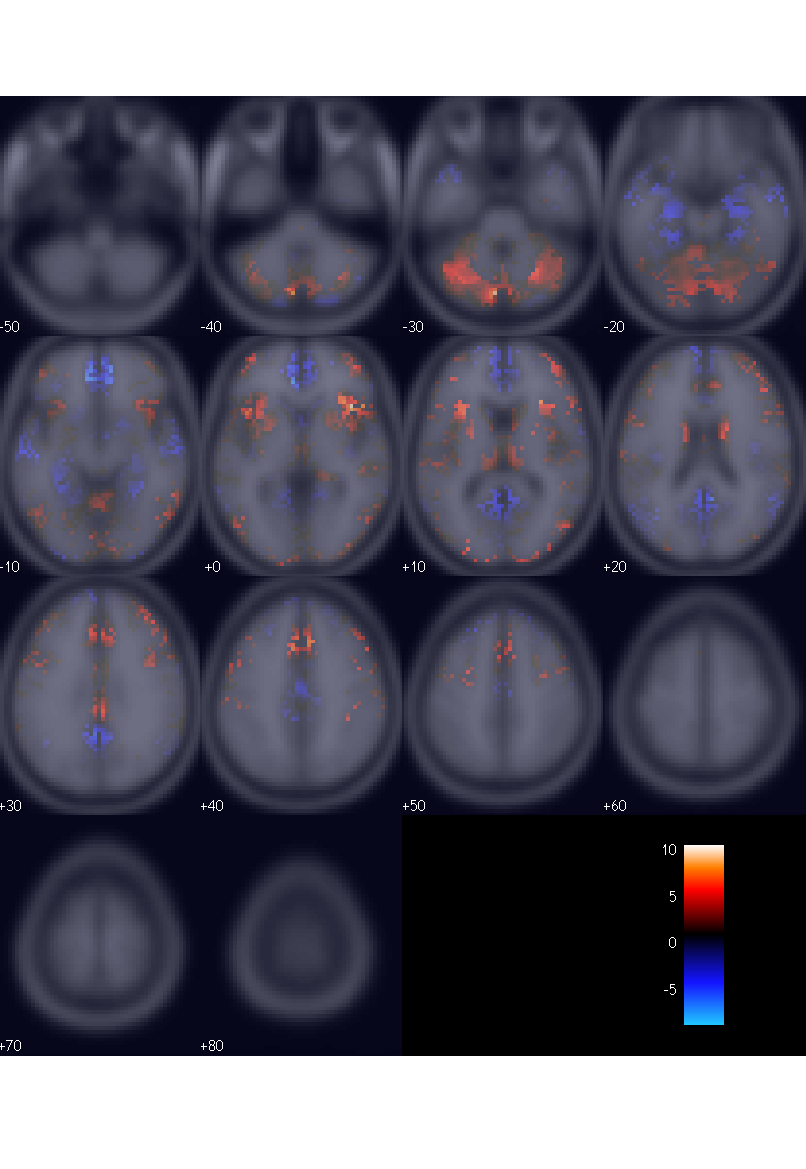
\includegraphics{f_map_gl_raw_t}
    \centering
	\caption{(Raw, that is unthresholded, $t$-values for all trials in the stimulus-response learning task (i.e. part 2), compared to the rest period,  overlaid onto the T1 MNI-352 template.   Each number is the height of the axial slice in MNI space.}
	\label{fig:glraw}
\end{figure}

\begin{figure}[tp]
	\fitfigure{f_map_gxl_p05}
    \centering
	\caption{Statistical parametric map for all trials in the stimulus-response learning task (i.e. part 2) examining the interaction between gains and losses.  \emph{Left} is a glass brain, showing all significant clusters mapped down to 3 two dimensional representations.  \emph{Right} is a set of axial slices highlighting strong areas of activity overlaid onto the T1 MNI-352 template.  $Z$ is the height of the axial slice in MNI space.}
	\label{fig:gxl}
\end{figure}

\subsection{Regions and models}
\label{sub:regoins}
\subsubsection{The right chunks}
\label{subsub:chunks}
Following whole-brain analysis, regions of interest were selected using two methods, that were later compared.  The first employed only regions from the Harvard-Oxford probabilistic anatomical atlas, using the 50\% cutoff \cite{Desikan:2006p9370}.  The second combined anatomical regions with functional clusters isolated using both sets of data collected during the second half of part 1 and from the reward category localizer.  Analyses showed the clustered regions and entire anatomical regions displayed very similar model-fits.  So to limit the complexity of later analyses, and to increase power, functional analyses were dropped in favor of the larger anatomical regions.  Anatomical regions of interest were selected \emph{a priori} based on previous studies of reinforcement and category learning (see the \emph{Introduction for a review}).  Left and right subcortical regions of interest were the dorsal caudate, ventral striatum/nucleus accumbens, hippocampus, and amygdala.   Bilateral cortical areas were the middle frontal cortex (i.e. dorsal lateral PFC), superior frontal cortex (which contains ventral medial PFC), orbital frontal cortex, anterior and posterior cingulate (ACC and PCC for short).

% -- PROOFED ABOVE
\subsubsection{A Way To(o) Many}
\label{subsub:tomany}
In total there 6 models under evaluation -- the three kinds of similarity adjustment, (``none'', ``exp'', and ``gauss''), with two possible reward codes (``acc'' and ``gl'').  With the two terms of interest (i.e. value and the reward prediction error) that is 12 comparisons.  The are also a number of \emph{a priori} confounds to our signals of interest: the similarity metrics, the reward codes, and the grating parameters.  Bringing the total to 23.  However the models are not nested\footnote{

    Often defined by whether or not tow models can be made identical by adding or subtracting parameters \cite{Forster:2000p9623}} and so are not amenable to $F$-tests, the common statistical way to compare model fits.  Further complicating the issue is the fact that each of the models is covariate, if not collinear, with the others.  To top it off, none of the three are statistically independent; Reinforcement learning can viewed as a regression of the reward code onto behavioral choices.  All these factors combined would make statistical testing difficult, to say the least.  But fortunately finding \emph{the} best model is not the goal.  

The latest recordings of phasic (i.e. reward prediction) activity in the VTA/SNc suggests a complicated reward and prediction error coding scheme (see p\pageref{subsub:expectations}), wherein several separate sets of calculations may be carried out independently \cite{Kim:2006p1063, Matsumoto:2009p7219, Smith:2011p8133}.  The observed BOLD signal is then an aggregate of these many activities. It is likely then  that more than one of the models is correct, making null hypothesis significance tests an incorrect choice.  Model selection is the right choice.

Model selection is the process finding a \emph{family} of models/variates that best predict a given dataset \cite{Rao:2001p9457}, with most techniques trying to wisely balance parsimony with increasing fit (i.e. solving the bias versus variance dilemma \cite{Geman:1p9469}).  Unfortunately most model selection techniques require assumptions the models cannot meet (e.g. statistical independence).  The few that can tend to be complex recent statistical inventions.  And rather than navigate the those troubled and unproven waters, I took a simpler approach, simply examining each model independently and ranking them.

A score (AIC, Akaike Information Criterion \cite{Akaike:1974p9530}) was assigned to each of the models/codes for every participant and region of interest.  The absolute AIC score across participants is not however meaningful.  Only the relative values are of interest \cite{Wagenmakers:2004p9472}.  Individual's scores were normalized and ranked by subtracting from each from the best (lowest) score \cite{Anderson:2000p9475}. The normalized set was then transformed to Akaike Weights, a way to easily compare the conditional probabilities of each model being true \cite{Wagenmakers:2004p9472}.  The Akaike Weights were then averaged across participants for each model and region of interest.

\subsubsection{Information on Information}
\label{subsub:way}
AIC is a measure of loss; how much information is lost by substituting the model for the true distribution, i.e. the data.  The lower the AIC score, the better the model.  Unlike null hypothesis tests and Bayesian measures, AIC-based methods do not seek to find \emph{a} truth, but instead serve to rank models.  AIC offers then only relative insight, and is unable to make any claims about absolute significance.  Significance is a separate question, one I'll return to later.  Besides this limitation, AIC has some significant advantages. Five are reviewed below.

One, unlike maximum-likelihood AIC is designed to a be parsimonious score.  It penalizes for additional parameters.  It may therefore choose a worse model (as measured by likelihood or mean squared error) over a better but more complex one. This is the essence of Occam's razor\footnote{Famously and pithily expressed as, ``Entities are not to be multiplied beyond necessity''.}. 

Two, it fits with the process of science.  When designing an experiment it is rare that there are only two possible outcomes, instead typically there are several competing hypothesis, some of which may not be mutually exclusive.  AIC's focus on relative differences, and evidential weights, meshes perfectly with the reality of multiple working hypotheses \cite{Burnham:2004p9621}.

Three, truth can remain elusive.  A common alternative to AIC is BIC, the Bayesian Information Criterion.  Like AIC, BIC is derived from the log-likelihood of a model, however its derivation requires a rather strict (and often unrealistic) assumption -- that the true model is among the candidates \cite{Forster:2000p9623}.  And while it may be philosophically debatable whether any mathematical model can \emph{completely} describe reality, in this study it is I know my models are incomplete.  As, one, the human reinforcement learning literature contains several recent theoretically unaccounted for findings and, two, there are theoretical developments I do not include here to keep the models tractable (see the \emph{Introduction} for a review).  

Four, AIC values are easily interpretable once they're transformed to Akaike Likelihoods or Weights\footnote{
    Likelihood for model $k$ among $K$ working hypotheses/models is given by $L_k = e^{-0.5({AIC}_k - {min}_{K}{(AIC)})}$, which is then normalized, becoming an Akaike Weight by $w_k = L_k / \sum\limits_{k=1}^K L_k$ \cite{Burnham:2004p9621}.}.  The likelihood is simply the likelihood the model is correct (based on the information loss associated with it), while the Akaike Weights are just normalized likelihoods.  As the Weights sum to one, the conditional likelihood of one model compared to another is just the ratio of their weights \cite{Burnham:2004p9621}.  For example, the conditional likelihood of model A over model B is just $w_A/w_B$.  That is, the likelihoods and Akaike Weights are intrinsically measures of effect size \cite{Anderson:2000p9475,Forster:2000p9623}.  Despite the fact that it is often used to express the likelihood of correctly rejecting the null hypothesis, the $p$ value is not a measure of effect, as $p$ is contingent not just on effect size but on sample number.  
    
    Five, AIC has a history with models of categorization. \citeNP{McKinley:1996p9532,Maddox:2001p9533}, among several others, used AIC to compare behavioral results to several alternative models of categorization.  

\subsubsection{F-Them}
\label{subsub:F}
AIC ranks offer no information on significance, in the familiar null hypothesis sense, or on the absolute fit of the model.  I addressed both of these in a series of $F$-tests run prior to AIC analysis.  These (fixed-effect, across participant) ominbus tests asked whether the total set of regression parameters for each linear model (described below) could explain the BOLD time series better than chance, i.e could the null hypothesis (of 0) be rejected.  Keeping with recommendations of \citeNP{Burnham:2004p9621, Forster:2000p9623}, who argue that as AIC and significance tests are so dissimilar that direct comparison/interaction between them them will be at best misleading, the models are not discarded based on significance.  All models are retained, and later AIC ranked.  The $F$-tests are a separate measure whose results are integrated during interpretation, not during model selection.

\subsubsection{Code, BOLD, and Models.}
\label{sub:cmb}
A total of 23 models were compared for each of the 16 regions of interest for each of the 16 subjects, 5888 comparisons in total.  Each of the models is described below (Table 1).  In general, a time-series (e.g the reward prediction error for each trial or the similarity for that trial's outcome) was convolved with a ``canonical''  haemodynamic response function, a mixture of gamma functions that serves as a parsimonious estimate of the (instantaneous) BOLD response \cite{Friston:1998p2022}.  The convolved series was then low-pass filtered, matching the treatment of the BOLD data (p\pageref{subsub:preprocessed}).  Each convolved and filtered model was then regressed onto the BOLD response for each participant's region of interest, retaining all parameters and fit measures inside subject-level HDF5 files (\url{http://www.hdfgroup.org/HDF5/}).  

No available fMRI analysis package returns AIC scores (or measures that could be converted to such) and none allow for the efficient (i.e programmatic) analysis of many competing computational models. So I created a roi-focused fMRI data analysis tool in Python (v2.7.1) to meet those two needs.  This module, simply named ``roi'', has since been release under the BSD license and is available for download at \url{https://github.com/andsoandso/roi}. It relies on the nibabel library to read the nifiti-1 files  (v1.2.0; \url{http://nipy.org/nibabel}), nitime for timeseries analysis, (v0.4; \url{http://nipy.sourceforge.net/nitime/}) Numpy for generic numerical work (v1.6.1; \url{http://numpy.scipy.org/}), with the GLS function from the scikits.statsmodels module handling the regerssions (v0.40; \url{http://statsmodels.sourceforge.net/}).  Model-to-BOLD fit parameters, as well as other useful metadata, was then extracted and stored in text files suitable for importing into R (v2.15.1; \url{http://www.r-project.org/}).  All plotting and model ranking (as well as the $F$-tests) were carried out in R.  For complete BSD licensed code see, \url{https://github.com/andsoandso/fmri/tree/master/catreward/roi/results}.

\subsubsection{Our Kinds of Models}
\label{subsub:ourkinds}
To simplify visualization and analysis, each of the models was classified into one of 5 families.  Family one, denoted ``boxcar'', was identical to that first used in the whole-brain analysis (p\pageref{sub:blob}) -- all trials versus the rest condition.  This is a univariate time-series that predicts no trial-specific effects; No matter the task the brain, thus the BOLD response, just flicks on then off.  It serves as a useful standard against which to compare the model-based regressors.  The next two families were controls (i.e. \emph{a priori} covariates), with the similarity metrics and grating parameters grouped into one family (``control\_similarity'') and the reward codes (both raw and similarity adjusted) into the other (``control\_reward'').  The fourth family was all the reward prediction errors (``rpe'').  The fifth was the value estimates (``value'').

\begin{center}
    \begin{longtable}{ | l | l | l | p{6cm} |}
    \caption{All models, their designations (Codes), families, and descriptions.}\\
    \hline
    Number & Code & Family & Description \\ \hline
         1 & 0\_1 & boxcar & The simplest model, a univariate analysis of all conditions. \\ \hline
         2 & acc & control\_reward & Behavioral accuracy. \\ \hline
         3 & acc\_exp & control\_reward & Behavioral accuracy, diminished by (exponential) similarity. \\ \hline
         4 & acc\_gauss & control\_reward & Behavioral accuracy, diminished by (Gaussian) similarity. \\ \hline
         5 & gl & control\_reward & Gains and losses. \\ \hline 
         6 & gl\_exp & control\_reward & Gains and losses, diminished by (exponential) similarity. \\ \hline
         7 & gl\_gauss & control\_reward & Gains and losses, diminished by (Gaussian) similarity. \\ \hline
         8 & rpe\_acc & rpe & Reward prediction error - derived from accuracy. \\ \hline
         9 & rpe\_acc\_exp & rpe & Reward prediction error - derived from accuracy diminished by (exponential) similarity. \\ \hline
        10 & rpe\_acc\_gauss & rpe & Reward prediction error - derived from accuracy diminished by (Gaussian) similarity. \\ \hline
        11 & value\_acc & value & Value - derived from accuracy. \\ \hline
        12 & value\_acc\_exp & value & Value - derived from accuracy diminished by (exponential) similarity. \\ \hline
        13 & value\_acc\_guass & value & Value - derived from accuracy diminished by (Gaussian) similarity. \\ \hline
        14 & rpe\_gl & rpe & Reward prediction error - derived from gains and loses. \\ \hline
        15 & rpe\_gl\_exp & rpe & Reward prediction error - derived from gains and losses diminished by (exponential) similarity. \\ \hline
        16 & rpe\_gl\_gauss & rpe & Reward prediction error - derived from gains and losses diminished by (Gaussian) similarity. \\ \hline
        17 & value\_gl & value & Value - derived from gains and losses. \\ \hline
        18 & value\_gl\_exp & value & Value - derived from gains and losses diminished by (exponential) similarity. \\ \hline
        19 & value\_gl\_gauss & value & Value - derived from gains and losses diminished by (Gaussian) similarity. \\ \hline 
        20 & exp & control\_similarity & Outcome similarity (exponential). \\ \hline
        21 & gauss & control\_similarity & Outcome similarity (Gaussian). \\ \hline
        22 & angle & control\_similarity & Grating angle parameter. \\ \hline
        23 &width & control\_similarity & Grating width parameter. \\ \hline
    \end{longtable}
\end{center}


\subsection{Model Results}
\label{sub:modelresults}
I'll work through the many results first by subcortical areas then move on to the cortical.  The general analysis strategy was to first find the top family, indicated by the largest family-average Akaike Weight.  I then examined the next highest scoring to family to see if it was close (less the 1.5 times as likely) to the top.  If it was both, families were included.  I then examined the relative likelihood of each model in the top family/families.  Within-family models that were about $\ge$1.5 times more likely then their neighbor were dubbed ``substantively more informative''.  Like the significance thresholded in null hypothesis tests this $\ge$1.5 is an arbitrary threshold.  However in order discuss and interpret these results a line must be drawn between meaningful and not, and $\ge$1.5 is a good minimum cutoff \cite{Anderson:2000p9475, Forster:2000p9623}.  As I stated though at the outset, more than one model may be right.  Thus the threshold was treated a loose cutoff.  To get sense of overall model quality, I also calculated the likelihood of the best model over the boxcar (i.e. the non-parametric standard).  Finally I examined all models, not just the top family, for any outliers that may have scored well despite their families overall poor performance.  Cases with these kinds of outliers were restricted to regions who, as judged by $F$-tests, were not good absolute models.  So these outliers are probably just noise.  Still, a couple surprising outliers are noted just in case they're meaningful after all.

Still as this is the first attempt of this kind to AIC-rank models of fMRI data, and while I put much thought and research into the above scheme, it may be flawed.  It is also arbitrary (beyond the $\ge$1.5 cutoff); Why not discuss the top 3, or 4 families, or even just include them all?  To attempt then to minimize the effect of these arbitrary, but necessary, decisions the complete set of models (and $F$-tests) are included for every region of interest.


\subsubsection{From up high}
\label{subsub:fromuphigh}
For 10 of the 16 regions of interest the ``rpe'' family scored highest.  Of these 10, 8 were similarity-adjusted (6/8 were Gaussian).  The next best family was ``control\_similarity'' with 3 regions, followed by ``boxcar'' with another 3.  Notably, ``value'' was not the most informative model family for any region of interest, and indeed the one region (ACC) for which it was second, ``rpe'' was 1.8 times more likely.


\subsubsection{Under Cortical}
\label{subsub:belowctx}
In the dorsal caudate (Figure~\ref{fig:caudate}), only the ``rpe'' family offered a more informative fit that the ``boxcar'', being 2.61 times more likely in the left and 2.85 in the right.  Bilaterally, and using the acc coding scheme, the Gaussian similarity-adjusted model (i.e. ''rpe\_acc\_gauss'') was substantively more informative than the either unadjusted model (``rpe\_acc'' -- left/right: 1.45/1.54 or ``rpe\_gl'' 1.82, \emph{right}: 1.70).  Surpsingly, given its similarity ot the Gaussian adjustment, the ``rpe\_acc\_exp'' scored no better than the unadjusted.  In what will become a reoccurring theme, all models were significant bilaterally in the dorsal caudate (Figure~\ref{fig:fvalcaudate}).  And while the $F$-values themselves to some degree mimic the patterns of the Akaike Weight, it would not be possible to reliably disassociate them given the slight relative differences.


\begin{figure}[tp]
	\fitfigure{f_meanbar_run4_c_aic_w_bilat_Caudate}
    \centering
    \caption{Dorsal caudate (left and right) -- Akaike Weights for all models.  Colors indicate model family (see p\pageref{sub:cmb} for details). Bars represent standard errors.}
	\label{fig:caudate}
\end{figure}
\begin{figure}[tp]
	\fitfigure{f_plot_run4_c_fvalue_bilat_Caudate}
    \centering
    \caption{Dorsal caudate (left and right) -- $F$-values for all models.  Significance is the $p <$ 0.05 level, trend is between $p <$ 0.05 and 0.10.  Colors indicate model family (see p\pageref{sub:cmb} for details).}
	\label{fig:fvalcaudate}
\end{figure}


% -- Subcortical
\begin{figure}[tp]
	\fitfigure{f_meanbar_run4_c_aic_w_bilat_Accumbens}
    \centering
    \caption{Nucleus Accumbens (left and right) -- Akaike Weights for all models.  Colors indicate model family (see p\pageref{sub:cmb} for details). Bars represent standard errors.}
	\label{fig:accumbens}
\end{figure}
\begin{figure}[tp]
	\fitfigure{f_plot_run4_c_fvalue_bilat_Accumbens}
    \centering
    \caption{Nucleus accumbens (left and right) -- $F$-values for all models.  Significance is the $p <$ 0.05 level, trend is between $p <$ 0.05 and 0.10.  Colors indicate model family (see p\pageref{sub:cmb} for details).}
	\label{fig:fvalaccumbens}
\end{figure}


\begin{figure}[tp]
	\fitfigure{f_meanbar_run4_c_aic_w_bilat_Amygdala}
    \centering
    \caption{Amygdala (left and right) -- Akaike Weights for all models.  Colors indicate model family (see p\pageref{sub:cmb} for details). Bars represent standard errors.}
	\label{fig:amygdala}
\end{figure}
\begin{figure}[tp]
	\fitfigure{f_plot_run4_c_fvalue_bilat_Amygdala}
    \centering
    \caption{Amygdala (left and right) -- $F$-values for all models.  Significance is the $p <$ 0.05 level, trend is between $p <$ 0.05 and 0.10.  Colors indicate model family (see p\pageref{sub:cmb} for details).}
	\label{fig:fvalamygdala}
\end{figure}


\begin{figure}[tp]
	\fitfigure{f_meanbar_run4_c_aic_w_bilat_Hippocampus}
    \centering
    \caption{Hippocampus (left and right) -- Akaike Weights for all models.  Colors indicate model family (see p\pageref{sub:cmb} for details). Bars represent standard errors.}
	\label{fig:hippocampus}
\end{figure}
\begin{figure}[tp]
	\fitfigure{f_plot_run4_c_fvalue_bilat_Hippocampus}
    \centering
    \caption{Hippocampus (left and right) -- $F$-values for all models.  Significance is the $p <$ 0.05 level, trend is between $p <$ 0.05 and 0.10.  Colors indicate model family (see p\pageref{sub:cmb} for details).}
	\label{fig:fvalhippocampus}
\end{figure}

\subsubsection{On that thinkin' sheet}
\label{subsub:onsheet}
Now discuss the cortical results....

\clearpage
% -- Cortex!
\begin{figure}[tp]
	\fitfigure{f_meanbar_run4_c_aic_w_Cingulate_Gyrus_anterior_division}
    \centering
    \caption{ACC -- Akaike Weights for all models.  Colors indicate model family (see p\pageref{sub:cmb} for details). Bars represent standard errors.}
	\label{fig:ant}
\end{figure}
\begin{figure}[tp]
	\fitfigure{f_plot_run4_c_fvalue_Cingulate_Gyrus_anterior_division}
    \centering
    \caption{ACC -- $F$-values for all models.  Significance is the $p <$ 0.05 level, trend is between $p <$ 0.05 and 0.10.  Colors indicate model family (see p\pageref{sub:cmb} for details).}
	\label{fig:fvalant}
\end{figure}


\begin{figure}[tp]
	\fitfigure{f_meanbar_run4_c_aic_w_Cingulate_Gyrus_posterior_division}
    \centering
    \caption{PCC -- Akaike Weights for all models.  Colors indicate model family (see p\pageref{sub:cmb} for details). Bars represent standard errors.}
	\label{fig:post}
\end{figure}
\begin{figure}[tp]
	\fitfigure{f_plot_run4_c_fvalue_Cingulate_Gyrus_posterior_division}
    \centering
    \caption{PCC -- $F$-values for all models.  Significance is the $p <$ 0.05 level, trend is between $p <$ 0.05 and 0.10.  Colors indicate model family (see p\pageref{sub:cmb} for details).}
	\label{fig:fvalpost}
\end{figure}


\begin{figure}[tp]
	\fitfigure{f_meanbar_run4_c_aic_w_Frontal_Medial_Cortex}
    \centering
    \caption{Frontal (ventral) medial PFC -- Akaike Weights for all models.  Colors indicate model family (see p\pageref{sub:cmb} for details). Bars represent standard errors.}
	\label{fig:vmpfc}
\end{figure}
\begin{figure}[tp]
	\fitfigure{f_plot_run4_c_fvalue_Frontal_Medial_Cortex}
    \centering
    \caption{Frontal (ventral) medial PFC -- $F$-values for all models.  Significance is the $p <$ 0.05 level, trend is between $p <$ 0.05 and 0.10.  Colors indicate model family (see p\pageref{sub:cmb} for details).}
	\label{fig:fvalvmpfc}
\end{figure}


\begin{figure}[tp]
	\fitfigure{f_meanbar_run4_c_aic_w_Frontal_Orbital_Cortex}
    \centering
    \caption{Orbital frontal cortex -- Akaike Weights for all models.  Colors indicate model family (see p\pageref{sub:cmb} for details). Bars represent standard errors.}
	\label{fig:ofc}
\end{figure}
\begin{figure}[tp]
	\fitfigure{f_plot_run4_c_fvalue_Frontal_Orbital_Cortex}
    \centering
    \caption{Orbital frontal cortex -- $F$-values for all models.  Significance is the $p <$ 0.05 level, trend is between $p <$ 0.05 and 0.10.  Colors indicate model family (see p\pageref{sub:cmb} for details).}
	\label{fig:fvalofc}
\end{figure}


\begin{figure}[tp]
    \fitfigure{f_meanbar_run4_c_aic_w_Insular_Cortex}
    \centering
    \caption{Insula -- Akaike Weights for all models.  Colors indicate model family (see p\pageref{sub:cmb} for details). Bars represent standard errors.}
	\label{fig:insula}
\end{figure}
\begin{figure}[tp]
	\fitfigure{f_plot_run4_c_fvalue_Insular_Cortex}
    \centering
    \caption{Insula -- $F$-values for all models.  Significance is the $p <$ 0.05 level, trend is between $p <$ 0.05 and 0.10.  Colors indicate model family (see p\pageref{sub:cmb} for details).}
	\label{fig:fvalinsula}
\end{figure}


\begin{figure}[tp]
	\fitfigure{f_meanbar_run4_c_aic_w_Middle_Frontal_Gyrus}
    \centering
    \caption{Middle frontal (dorsal-lateral) PFC -- Akaike Weights for all models.  Colors indicate model family (see p\pageref{sub:cmb} for details). Bars represent standard errors.}
	\label{fig:dlpfc}
\end{figure}
\begin{figure}[tp]
	\fitfigure{f_plot_run4_c_fvalue_Middle_Frontal_Gyrus}
    \centering
    \caption{Middle frontal (dorsal-lateral) PFC -- $F$-values for all models.  Significance is the $p <$ 0.05 level, trend is between $p <$ 0.05 and 0.10.  Colors indicate model family (see p\pageref{sub:cmb} for details).}
	\label{fig:fvaldlpfc}
\end{figure}

\clearpage
\newpage
\bibliography{bibmin}
%%%%%%%%%%%%%
\end{document}
%%%%%%%%%%%%%
